\section{Algorithmic extensions to SEP}
%
SEP has been motivated from a practical perspective by the limitations inherent in EP and ADF. In this section we extend SEP in four orthogonal directions and through these extensions relate SEP to SVI. Many of the algorithms described in this section are summarised in Figure \ref{fig:relationship-algorithms} and they are detailed in the following discussions.

\begin{figure}
\centering
\def\svgwidth{1\linewidth}
%\subfigure[\label{fig:relationship-algorithms}]{
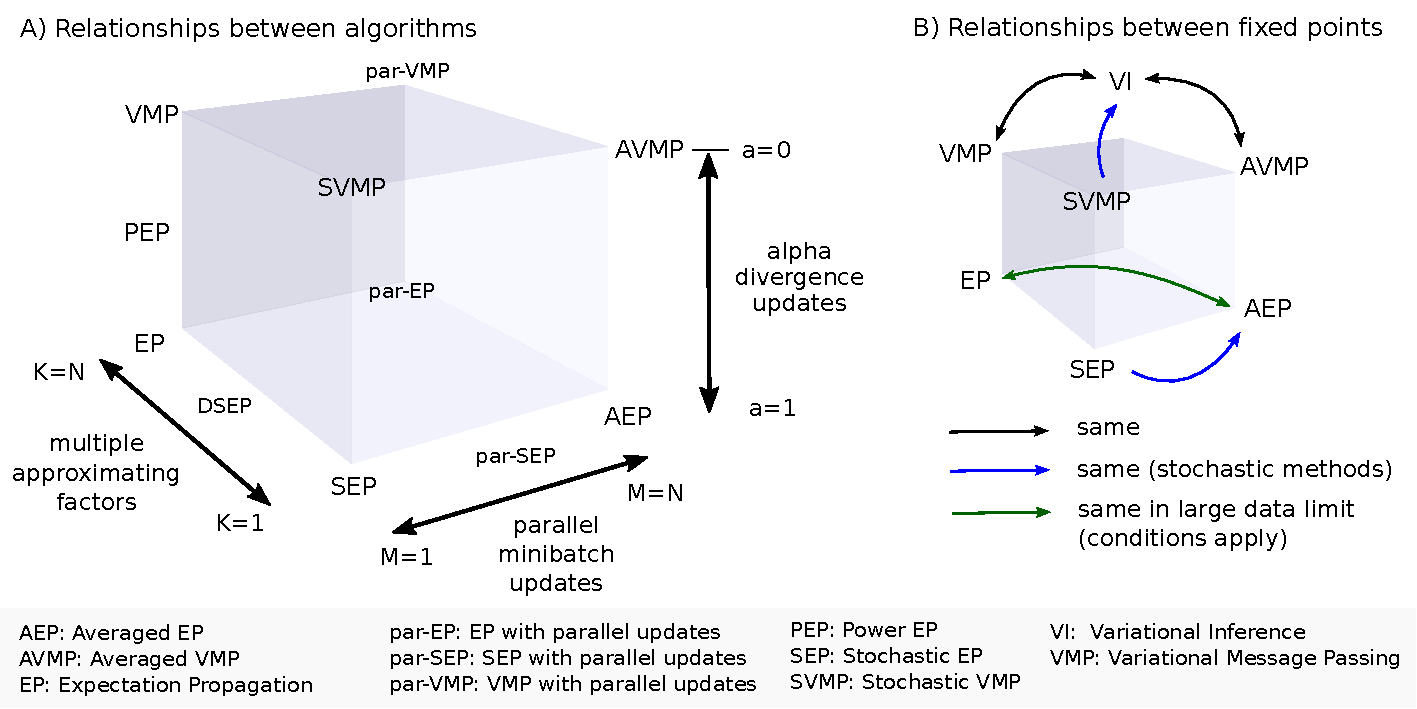
\includegraphics[height=6.5cm]{Chapter3/sep/fig/relationship-algorithms.pdf}%}
\caption{Relationships between algorithms. Note that care needs to be taken when interpreting Minka's alpha-divergence as $a \rightarrow 0$. See the main text for further discussions.}
\label{fig:relationship-algorithms}
\end{figure}

%
\subsection{Parallel SEP: relating the EP fixed points to SEP}
%

The SEP algorithm outlined above approximates one likelihood at a time which can be computationally slow. However, it is simple to parallelise the SEP updates by following the same recipe by which EP is parallelised. Consider a minibatch comprising $M$ datapoints (for a full parallel (batch) update use $M=N$). First we form the cavity distribution for each likelihood. Unlike EP these are all identical. Next, in parallel, compute $M$ intermediate factors $f_m(\mparam) \leftarrow \mathtt{proj}[\tilde{p}_m(\mparam)] / q_{-1}(\mparam)$. In EP these intermediate factors become the new likelihood approximations and the approximation is updated to $q(\mparam) = p_0(\mparam) \prod_{n \ne m} f_n(\mparam) \prod_{m} f_m(\mparam) $. In SEP, the same update is used for the approximating distribution, which becomes $q(\mparam) \leftarrow p_0(\mparam) f_{old}(\mparam)^{N-M} \prod_{m} f_m(\mparam) $ and, by implication, the approximating factor is $f_{new}(\mparam) = f_{old}(\mparam)^{1-M/N} \prod_{m=1}^M f_m(\mparam)^{1/N}$. One way of understanding parallel SEP is as a double loop algorithm. The \emph{inner loop} produces intermediate approximations  $q_m(\mparam) \leftarrow \arg\min_q \mathrm{KL}[\tilde{p}_m(\mparam) ||q(\mparam)]$; these are then combined in the \emph{outer loop}: $q(\mparam) \leftarrow \arg\min_q \sum_{m=1}^M \mathrm{KL}[q(\mparam) ||q_m(\mparam)] + (N-M) \mathrm{KL}[q(\mparam) || q_{old}(\mparam)]$.
%

For $M=1$ parallel SEP reduces to the original SEP algorithm. For $M=N$ parallel SEP is equivalent to the so-called Averaged EP (AEP) algorithm proposed in a concurrent work \citep{dehaene:aep2015,dehaene:aep2018} as a theoretical tool to study the convergence properties of normal EP. This work showed that when using Gaussian approximations, under fairly restrictive conditions,\footnote{e.g.~log likelihood functions that are smooth with bounding conditions up to the 4th-order derivative, although this is not a necessary condition.} AEP converges to the same fixed points as EP in the large data limit ($N \rightarrow \infty$).

There is another illuminating and arguably more direct connection between SEP and AEP. Since SEP's approximating factor $f(\mparam)$ converges to the geometric average of the intermediate factors $\bar{f}(\mparam) \propto [\prod_{n=1}^N f_n(\mparam)]^{\frac{1}{N}}$, SEP converges to the same fixed points as AEP, and therefore under certain conditions \citep{dehaene:aep2015,dehaene:aep2018}, to the same fixed points as EP. In practice decreasing learning rates, e.g. $\{\epsilon_t\}$ satisfying the Robbins and Monro criterion \citep{robbins:stochastic1951} $\sum_t \epsilon_t = \infty$, $\sum_t \epsilon_t^2 < \infty$, may be used to achieve convergence.
%
It is possible that there are more direct relationships between EP and SEP's dynamics, but that is still an open question.

\subsection{Stochastic power EP: relationships to variational methods}
The SEP algorithm generalises to the power-EP case in a straight-forward manner. Instead of removing one copy of the tied factors in Algorithm \ref{alg:sep}, when power $\alpha$ is in use we remove $\alpha$ fraction of the tied factors:
$$q_{-\alpha} \propto q(\mparam) / f(\mparam)^{\alpha}.$$
The moment matching step proceeds as in the power EP algorithm, precisely, 
$$f_n(\mparam)^{\alpha} \leftarrow \mathrm{proj}[ q_{-\alpha}(\mparam) p(\x_n | \mparam)^{\alpha} ] / q_{-\alpha}(\mparam) .$$
Similar to the power-EP case, the projection operator becomes I-projection when setting $\alpha \rightarrow 0$.

%
%NEED A PASS-THROUGH AGAIN
The relationship between variational inference and stochastic variational inference \citep{hoffman:svi2013} mirrors the relationship between EP and SEP. 
%
Can these relationships be made more formal? In the following we show that, if the moment projection step in EP is replaced by a natural parameter matching step (i.e.~I-projection) then the resulting algorithm is equivalent to the Variational Message Passing (VMP) algorithm \citep{winn:vmp2005, minka:divergence2005}. 

We first briefly sketch the VMP algorithm using the EP framework but replacing the moment matching step with natural parameter matching. We assume the approximate posterior $q(\mparam)$ is in some exponential family: 
\begin{equation}
q(\mparam) \propto \exp \left[ \langle \bm{\lambda}_q, \bm{\Phi}(\mparam) \rangle \right].
\end{equation}
At time $t$ we have the current estimate of the natural parameter $\bm{\lambda}_q^t$, which is defined as the sum of local variational parameters:
%
$\bm{\lambda}_q^t \buildrel\triangle\over = \bm{\lambda}_0 + \sum_{n=1}^N \bm{\lambda}_n^t$.\footnote{This notation implicitly assumes that the prior also belongs to the approximate distribution family $\mathcal{Q}$. In general we can propose another factor to approximate $p_0(\mparam)$, and our result still applies.}
%
Here $\bm{\lambda}_0$ represents the natural parameter of the prior distribution $p_0(\mparam)$. VMP iteratively computes the update of each local estimate $\bm{\lambda}_n^{t+1}$ in the following procedure. First VMP computes the expected sufficient statistics $\hat{\bm{s}}_n$ about datapoint $\bm{x}_n$ using $\bm{\lambda}_q^t$, e.g.~$\hat{\bm{s}}_n = E_{q}[t(z_n, x_n)]$ in the original SVI paper \citep{hoffman:svi2013}. Then VMP forms the gradient by differentiating the variational lower-bound but with $q_{-1}(\mparam)$ as the prior:
\begin{equation}
\nabla_{\bm{\lambda}_q^t} \mathcal{L}_{\text{VI}} \propto \bm{\lambda}_{-1}^t + \hat{\bm{s}}_n - \bm{\lambda}_q^t, \quad
\bm{\lambda}_{-1}^t := \bm{\lambda}_q^t - \bm{\lambda}_{n}^t.
\end{equation}
Next VMP zeros the gradient and recovers the current update $\bm{\lambda}_n^{t+1} = \hat{\bm{s}}_n$. The stochastic version of VMP, if extended in a way as SEP is developed from EP, defines the global variational parameters as $\bm{\lambda}_q^t \buildrel\triangle\over = \bm{\lambda}_0 + N \bm{\lambda}^t$. It computes the expected sufficient statistics $\hat{\bm{s}}_n$ in the same way as VMP but changes the cavity to $\bm{\lambda}_{-1}^t = \bm{\lambda}_q^t - \bm{\lambda}^t$ in the variational lower-bound maximisation steps. Readers can verify that this returns the current update $\bm{\lambda}^{t+1} = \hat{\bm{s}}_n$ using the important fact that the local update (for example $\hat{\bm{s}}_n = E_{q}[t(z_n, x_n)]$) \emph{only} depends on the global parameter $\bm{\lambda}_q^t$. Now since we tie all the local updates, the global parameter update $\bm{\lambda}_q^{t+1} = \bm{\lambda}_0 + N \bm{\lambda}^{t+1} = \bm{\lambda}_0 + N \hat{\bm{s}}_n$. In practice we perform a damped update, where a typical choice of step size is $\epsilon = 1/N$ like in SEP:
\begin{equation}
\bm{\lambda}_q^{t+1} \leftarrow (1 - \frac{1}{N}) \bm{\lambda}_q^t + \frac{1}{N}(\bm{\lambda}_0 + N \bm{\lambda}^{t+1}) = \bm{\lambda}_0 + (N-1) \bm{\lambda}^t + \hat{\bm{s}}_n.
\end{equation} 

On the other hand, \cite{mandt:smoothedSVI2014} summarises SVI as to compute the current update by zeroing the gradient
\begin{equation}
\nabla_{\bm{\lambda}_q} \mathcal{L}_{\text{VI}} \propto \bm{\lambda}_0 + N \hat{\bm{s}}_n - \bm{\lambda}_q,
\end{equation}
which returns $\bm{\lambda}_q^{t+1} = \bm{\lambda}_0 + N \hat{\bm{s}}_n$ as well. This implies that SVI, when using learning rate $\epsilon = 1/N$, is equivalent to SVMP. 
%
More generally, the procedure can be applied any member of the PEP family of algorithms, but care has to be taken when taking the limiting cases $\alpha \rightarrow 0$.
%
These results lend weight to the view that SEP is a natural stochastic generalisation of EP.

\subsection{Distributed SEP: controlling granularity of the approximation}
\label{sec:chap3_sep_dep}
EP uses a fine-grained approximation comprising a single factor for each likelihood. SEP, on the other hand, uses a coarse-grained approximation comprising a signal global factor to approximate the average effect of all likelihood terms. One might worry that SEP's approximation is too severe if the dataset contains sets of data-points that have very different likelihood contributions (consider classifying handwritten digits into odd and even classes, for example). 
It might be more sensible in such cases to partition the dataset into $J$ disjoint pieces $\{ \data_j = \{\bm{x}_n\}_{n=N_{j-1}}^{N_j} \}_{j=1}^{J}$ with $N = \sum_{j=1}^J N_j$ and use an approximating factor for each partition. If normal EP updates are performed on the subsets, i.e.~treating $p(\data_j |\mparam)$ as a single true factor to be approximated, we arrive at the distributed EP (DEP) algorithm \citep{gelman:dep2014, xu:sms2014}, summarised in Algorithm \ref{alg:dep} and detailed as the following.

%But such updates are challenging as multiple likelihood terms must be included during each update necessitating additional approximations (e.g.~MCMC). 
%A simpler alternative uses SEP/AEP \textbf{inside} each partition, which implies a posterior approximation of the form $q(\mparam) \propto p_0(\mparam) \prod_{j=1}^J f_{j}(\mparam)^{N_j}$ with $f_{j}(\mparam)^{N_j}$ approximating $p(\data_j|\mparam)$. The limiting cases of this algorithm, when $J=1$ and $J=N$, recover SEP and EP respectively. 

%We have shown in the main paper that a proper design of data partitioning improves SEP's approximation accuracy. This distributed algorithm is inspired by the Distributed EP (DEP) algorithm \cite{gelman:dep2014, xu:sms2014} presented in Algorithm \ref{alg:dep}. 

After data partitioning, the posterior distribution and likelihood functions are denoted as
\begin{align}
p(\mparam|\data) &\propto p_0(\mparam) \prod_{j=1}^J p(\data_j|\mparam), \\
p(\data_j|\mparam) &= \prod_{\bm{x}_n \in \data_j} p(\bm{x}_n | \mparam).
\end{align}
%
Next DEP assigns factors to each sub-dataset likelihood, i.e.~$q(\mparam) \propto p_0(\mparam) \prod_{j = 1}^J F_j(\mparam)$ with each $F_j(\mparam)$ approximating $p(\data_j|\mparam)$. The projection step is no longer analytically tractable in general since the tilted distribution with multiple data-points often lacks a simple form. Instead DEP handles moment matching by nesting additional approximations, e.g.~MCMC, which might be undesirable in terms of time complexity figures.

How does the factor tying idea apply in this case? A naive implementation would simply tie the sub-dataset level factors, but one should notice that $N_j$ might not be equal for different subsets. Instead we still construct datapoint level approximate factors similar to SEP, i.e.~$q(\mparam) \propto p(\mparam) f(\mparam)^N$, but construct the update in DEP fashion. In other words, $N_j$ factors are replaced by the likelihood terms in the $j$th subset in order to form the tilted distribution. Later these $N_j$ copies are updated by exactly the same moment matching step as in DEP. We name this algorithm stochastic EP \emph{on} data partitions and to distinguish from another algorithm presented later we abbreviate it as stochastic distributed EP (SDEP) (see Algorithm \ref{alg:sdep}). It is trivial to parallelise this method just as one would do for DEP, and we abbreviate the corresponding version as ADEP. 

%
To have a deterministic\footnote{in the sense that the moment matching step does not employ Monte Carlo.} counterpart of DEP, we consider SEP/AEP \emph{inside} each partition. This strategy might be preferred when one wish to carve up the data and carry out deterministic inference routines distributed across machines. We name this approach as Distributed SEP/AEP (DSEP/DAEP). Different to both DEP and SDEP, the approximate posterior for DSEP is defined as $q(\mparam) \propto p_0(\mparam) \prod_j f_j(\mparam)^{N_j}$, with $f_j(\mparam)^{N_j}$ approximating $p(\data_j|\mparam)$. The computations are almost the same as SEP/AEP except that the updates only modifies the copies of the corresponded subset. This method is also detailed in Algorithm \ref{alg:dsep}, and the differences between the two factor tying proposals are also visualised in Figure \ref{fig:chap3_dsep_compare}.

In summary, a flexible class of EP-like approximate inference algorithms can be derived, by carving up the dataset and designing the approximating factor structures and update procedures. Computational complexity figures are further presented in Section \ref{sec:chap3_complexity} to allow selections of algorithms confronting computation constraints.

\begin{figure}[t]
% UGLY USE OF \vspace & \hspace follows
\begin{minipage}[t]{0.32\linewidth}
\centering
\begin{algorithm}[H] 
\caption{DEP} \small
\label{alg:dep} 
\begin{algorithmic}[1]
	\STATE compute cavity distribution \\$q_{-j}(\mparam) \propto q(\mparam) / F_j(\mparam)$ \\  
	\STATE compute tilted distribution \\$\tilde{p}_j(\mparam) \propto p(\data_j|\mparam) q_{-j}(\mparam)$
	\STATE moment matching: \\ \hspace{-5mm}$F_j(\mparam) \leftarrow \mathtt{proj}[\tilde{p}_j(\mparam)] / q_{-j}(\mparam) $ \\
\hspace{1mm}\\ \vspace{12.2mm} \hspace{1mm}\\
\end{algorithmic}
\end{algorithm}
\end{minipage}
%\quad
\begin{minipage}[t]{0.32\linewidth}
\centering
\begin{algorithm}[H]
\caption{SDEP} \small
\label{alg:sdep} 
\begin{algorithmic}[1] 
%\STATE initialize $\{\tilde{f}_a\}$

	\STATE compute cavity distribution \\ $q_{-j}(\mparam) \propto q(\mparam) / f(\mparam)^{N_j}$
	\STATE compute tilted distribution \\$\tilde{p}_j(\mparam) \propto p(\data_j|\mparam) q_{-j}(\mparam)$
	\STATE moment matching: \\\hspace{-6mm}$F_j(\mparam) \leftarrow \mathtt{proj}[\tilde{p}_j(\mparam)] / q_{-j}(\mparam) $
	\STATE inclusion:\\\hspace{-6mm}$f(\mparam) \leftarrow f(\mparam)^{1 - N_j / N} F_j(\mparam)^{1/N}$ \\
\hspace{1mm}\\ \vspace{2.7mm} \hspace{1mm}\\
\end{algorithmic}
\end{algorithm}
\end{minipage} 
%
\begin{minipage}[t]{0.33\linewidth}
\centering
\begin{algorithm}[H] 
\caption{DSEP} \small
\label{alg:dsep} 
\begin{algorithmic}[1] 
	\STATE compute cavity distribution \\$q_{-1}(\mparam) = q(\mparam) / f_j(\mparam)$
	\STATE choose a datapoint \\ $\bm{x}_n \sim \data_j$
	\STATE compute tilted distribution \\$\tilde{p}_j^{(n)}(\mparam) \propto p(\bm{x}_n|\mparam) q_{-1}(\mparam)$
	\STATE moment matching: \\\hspace{-9mm}$f_j^{(n)}(\mparam) \leftarrow \mathtt{proj}[\tilde{p}_j^{(n)}(\mparam)] / q_{-1}(\mparam)$
	\STATE inclusion:\\\hspace{-8mm} $f_j(\mparam) \leftarrow f_j(\mparam)^{1 - 1/N_j} f_j^{(n)}(\mparam)^{1/N_j}$
\end{algorithmic}
\end{algorithm}
\end{minipage}
%
\end{figure}
%
\begin{figure}[ht]
\centering
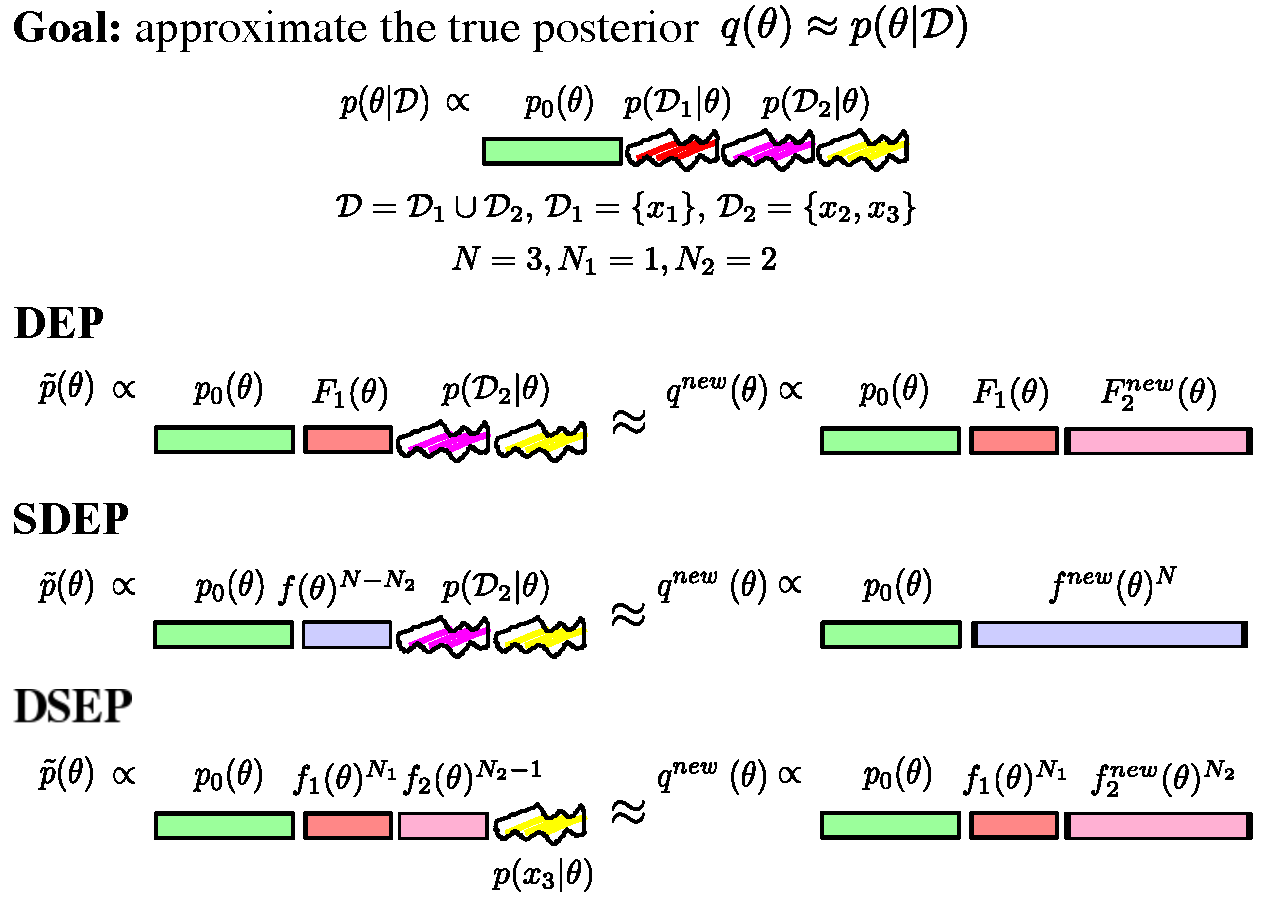
\includegraphics[width=1\linewidth]{Chapter3/sep/fig/dsep.pdf}
\caption{A cartoon visualisation on comparing DEP, SDEP and DSEP. One should notice that the definitions of $F_j(\mparam)$ in DEP is different from $f_j(\mparam)$ in DSEP. Here SDEP's moment matching step would typically require another approximate inference procedure, e.g.~simulating MCMC dynamics for a long time. On the other hand DSEP still use cheap updates computed on a single datum, which can be faster.}
\label{fig:chap3_dsep_compare}
\end{figure}

\subsection{SEP for latent variable models}

Many applications of EP involve latent variable models. Although this is not the main focus of the development, we show that SEP is applicable in this case and again it prevents the memory footprint from scaling with $N$. Critically as we shall see, the local factors $g_n(\z_n)$ do not need to be maintained in memory, although retaining them in memory might provide better initialisations that speeds up convergence potentially. This means that all of the advantages of SEP carry over to more complex models involving latent variables.

%
We consider a model containing latent variables $\z_n$ associated with each observation $\bm{x}_n$, which are drawn i.i.d.~from a prior $p_0(\z_n)$. SEP proposes approximations to the exact posterior over parameters and hidden variables 
\begin{equation}
p(\mparam, \{ \z_n\} | \data) \propto p_0(\mparam) \prod_n p_0(\z_n) p(\bm{x}_n | \z_n, \mparam)
\end{equation}
by tying the factors for the global parameter $\mparam$ but retaining the local factors for the hidden variables:
%
\begin{equation}
q(\mparam, \{ \z_n\}) \propto p_0(\mparam) f(\mparam)^N \prod_{n=1}^N g_n(\z_n) .
\end{equation}
In other words, SEP uses $f(\mparam) g_n(\z_n)$ to approximate $p(\bm{x}_n | \z_n, \mparam)p_0(\z_n)$.

Next we show a critical advantage of SEP for approximating latent variable posterior: the local factors $g_n(\z_n)$ do not need to be maintained in memory (again it might help to do so for better initialisation).
%
More formally, the cavity distribution is $q_{-n}(\mparam, \{ \z_n\}) \propto q(\mparam, \{ \z_n\})/(f(\mparam) g_n(\z_n)) $ and the tilted distribution is $$\tilde{p}_n(\mparam, \{ \z_n\}) \propto q_{-n}(\mparam, \{ \z_n\}) p(\bm{x}_n | \z_n, \mparam)p_0(\z_n).$$ This leads to a moment-update that minimises 
%
\begin{equation}
\mathrm{KL}[ p_0(\mparam) f(\mparam)^{N-1} p(\bm{x}_n | \z_n, \mparam)p_0(\z_n) \prod_{m\ne n} g_m(\z_m) || p_0(\mparam) f(\mparam)^{N-1} f'(\mparam) g_n(\z_n) \prod_{m\ne n} g_m(\z_m)] .\nonumber
\end{equation}
%
with respect to $f'(\mparam) g_n(\z_n)$. Importantly, the terms involving $\prod_{m\ne n} g_m(\z_m)$ are cancelled, meaning that these factors do not contribute to the local approximation step. For simple models the moments of $\z_n$ can be computed analytically given $q_{-1}(\mparam)$, thus $g_n(\z_n)$ is never stored in memory, resulting in a reduced memory footprint by a factor of $N$ again. 
%
It is also possible to have latent variables globally shared or shared in a data piece $\data_j$. But we can also extend SEP to these latent variables accordingly, which still provides computation gains in space complexity. In mathematical form, assume $\z_j$ a latent variable shared in $\data_j$. A prevalent example for this is the latent Dirichlet allocation (LDA) model \citep{blei:lda2003}, where $\data_j$ represents the $j^{\text{th}}$ document in the corpus and $\z_j$ represents the topic of the document. Then we construct $q(\z_j) \propto p_0(\z_j) g_k(\z_j)^{N_j}$ to approximate its posterior. This procedure still reduces memory by roughly a factor of $N/J$.
%

\vspace{1em}
\begin{tcolorbox}
\textbf{Remark} (amortised inference nested in SEP) \textbf{.}
In practice people may prefer maintaining the $g$ factors in memory, if the moment computation requires another optimisation inner-loop (which might be more expensive than the moment matching step itself). Examples of methods where this may be the case include latent Dirichlet allocation \citep{blei:lda2003} that has a hierarchy of latent variables, where VI methods also store variational $q$ distributions for some of the hidden variables. One potential recipe in this scenario is to apply amortised inference techniques, where in this case we can optimise the variational parameter $g_{\vparam}(\z_n | \x_n )$ for the factors attached to the latent variables. 
%Initial work with Vera Gangeskar Johne (for her Mphil thesis in Cambridge) on toy datasets suggested that this is a promising direction.
%
Another very closed related idea is to learn a model for the moments/messages passed in each SEP step with confidence estimates. A particular compelling feature of this approach is that one can control the use of the proposed message update by the model, and if rejected the algorithm can resort to the more expensive exact message computation using e.g.~MCMC. Interested readers are directed to \citep{heess:learning_messages2013, jitkrittum:kernel2015} for more details. 
\end{tcolorbox}

\section{Computational complexity}
\label{sec:chap3_complexity}
Besides the approximation accuracy, time and space complexities are also crucial for an efficient approximate inference algorithm to be widely-applicable, especially in systems that handle very large-scale datasets and also require fast computations. To provide a direct comparison between the methods discussed so far, we present the space and time complexity factors by considering Gaussian approximations with full covariance matrices. 

We assume an MCMC method is used for the DEP moment matching step, and assume it has time complexity $\mathcal{O}(H(n, D))$ if $n$ likelihood terms are involved and the random variable $\mparam$ is of dimension $D$, since it handles multiple likelihood functions at the same time for a single factor update. We also denote the time complexity factor of a normal EP moment matching step as $\mathcal{O}(h(D))$. Also since EP-like methods handle the natural parameters, for Gaussian approximations it requires $\mathcal{O}(D^3)$ time for matrix inversion and $\mathcal{O}(D^2)$ for matrix-vector multiplication in the inclusion step. By assumption EP's update step for a single factor can be done in a fast way, which means for a full pass through of the dataset $H(N, D) + D^3 + D^2 \geq N ( h(D) + D^3 + D^2)$. Furthermore in practice low-rank approximations can be applied to remove the $\mathcal{O}(D^3)$ factor if the random variable is very high dimensional, e.g.~see \cite{qi+minka:sparseGP2010} in EP literature. For the concern of memory usage, every factor in use occupies $\mathcal{O}(D^2)$ storage, although sparse approximations can significantly improve space complexity figures as well.

With all the above set-ups, we present the complexity figures in Table \ref{table:chap3_sep_complexity}, which apply to fully observed models, e.g.~Bayesian neural networks for classification tasks. Like the comparison between batch and stochastic learning methods, AEP-type methods produce more robust updates, and can be significantly faster than SEP-type methods if executed in parallel. However DEP/AEP algorithms require storing the factors in local worker machines, so in this regard SEP provides significant advantage in memory consumption in the price of slower convergence. 

\begin{table}[t]
\caption{Complexity figures for the EP algorithms discussed (with Gaussian approximations, full covariance matrices). The time complexity numbers are counted on a full pass of dataset, and the global approximations are updated after each moment computation. We assume the dataset is evenly split into $J$ disjoint subsets when applicable.}
\label{table:chap3_sep_complexity}
\begin{center}
\begin{tabular}{lll}
\multicolumn{1}{c}{\bf Algorithm}  &\multicolumn{1}{c}{\bf Time complexity} &\multicolumn{1}{c}{\bf Space complexity}
\\ \hline 
DEP (parallel)        	&$\mathcal{O}(D^3 + H(N/J, D) + D^2)$			&$\mathcal{O}(JD^2)$ \\
SDEP (sequel)        	&$\mathcal{O}(J(D^3 + H(N/J, D) + D^2))$			&$\mathcal{O}(D^2)$ \\
ADEP (parallel)        	&$\mathcal{O}(D^3 + H(N/J, D) + D^2)$			&$\mathcal{O}(JD^2)$ \\
DSEP (sequel)          &$\mathcal{O}(N(D^3 + h(D) + D^2))$ 		&$\mathcal{O}(D^2)$ \\
DAEP (parallel)         &$\mathcal{O}(J(D^3 + h(D) + D^2))$ 		&$\mathcal{O}(JD^2)$ \\
\hline
SEP 			         &$\mathcal{O}(N(D^3 + h(D) + D^2))$ 		&$\mathcal{O}(D^2)$ \\
AEP (parallel)		         &$\mathcal{O}(D^3 + h(D) + D^2)$ 		&$\mathcal{O}(ND^2)$ \\
ADF (multi.~pass) 		&$\mathcal{O}(N(h(D)))$ 		&$\mathcal{O}(D^2)$ \\
Normal EP         		&$\mathcal{O}(N(D^3 + h(D) + D^2))$ 		&$\mathcal{O}(ND^2)$ \\
\hline
Sampling 				&$\mathcal{O}(H(N, D))$			&$\mathcal{O}(D^2)$ \\
SVI 					&$\mathcal{O}(N(D^3 + \tilde{h}(D) + D^2))$	&$ \mathcal{O}(D^2)$ 
\end{tabular}
\end{center}
\end{table}

To conclude the discussion of computational efficiency we compare the complexity figures of SEP against those of SVI. Here we refer SVI to the general version which uses gradient descent, since the likelihood terms are very unlikely to be conjugate to the Gaussian approximation (thus the natural gradient descent algorithm \citep{hoffman:svi2013} does not apply). It is straightforward to see that both algorithms require the same amount of storage, which is $\mathcal{O}(D^2)$ in the Gaussian case. For the gradient descent update, as the gradient of the entropy term $\mathbb{H}[q]$ in the variational lower-bound requires computing the covariance matrix, this means the precision matrix as one of the natural parameters needs to be inverted. Therefore the cost for each gradient descent step in SVI is $\mathcal{O}(\tilde{h}(D) + D^3 + D^2)$, with $\mathcal{O}(D^3)$ the matrix inversion time, $\mathcal{O}(D^2)$ the update time for the precision matrix, and $\mathcal{O}(\tilde{h}(D))$ the computation time for the gradients of other terms in the variational lower-bound.
%
SVI might be more efficient in time complexity per iteration (i.e.~the runtime for processing one incoming observation, therefore $\tilde{h}(D) \leq h(D)$). However, as SEP uses fixed-point iterative updates, in practice SEP often converges in less passes of data than SVI thus is faster in total runtime, which is something that the above complexity analysis cannot take into account. For example \cite{hernandez-lobato:gp2016} showed that SEP, when applied to sparse GP classification, is significantly faster than SVI. SEP can be further accelerated using low-rank approximations when $D$ is large, which typically reduces the matrix inversion time to $\mathcal{O}(Dd^2)$ if we use rank-$d$ approximations.
